\documentclass{article}
\usepackage[top=2cm, bottom=2cm, left=2cm, right=2cm]{geometry}
\renewcommand{\thesubsection}{\thesection.\alph{subsection}}
\renewcommand{\thesubsubsection}{\thesubsection.\roman{subsubsection}}
\usepackage{subfiles}
\usepackage{gensymb}
\usepackage[numbered, framed]{mcode}
\usepackage{amsmath}
\usepackage{amssymb}
\usepackage{graphicx}
\usepackage{tikz}
\usetikzlibrary{shapes, shapes.multipart, shapes.geometric, arrows}
\graphicspath{{images/}}


%%gray = startstop; processes = orange, io files = purple, decisions = green, data variable/struct = cyan
\tikzstyle{arrow} = [thick,->,>=stealth]

\tikzstyle{startstop} = [circle, minimum width = 1cm, minimum height = 1cm, text centered,  draw=black, fill=gray!30]

\tikzstyle{io} = [trapezium, trapezium left angle=70, trapezium right angle=110, minimum width=2cm, minimum height=1cm, text centered, draw=black, fill=blue!30]

\tikzstyle{process} = [rectangle, minimum width = 3cm, minimum height = 1cm, text centered, draw=black, fill=orange!30]

\tikzstyle{filter} = [trapezium, trapezium left angle=110, trapezium right angle=110, minimum width=2cm, minimum height=1cm, text centered, draw=black, fill=orange!30]

\tikzstyle{filtersplit} = [trapezium, trapezium left angle=70, trapezium right angle=70, minimum width=2cm, minimum height=1cm, text centered, draw=black, fill=orange!30]

\tikzstyle{decision} = [diamond, minimum width=3cm, minimum height=1cm, text centered, draw=black, fill=green!30]

\tikzstyle{datastruct} = [rectangle, minimum width = 3cm, minimum height = 1cm, text centered, draw=black, fill=cyan!30]

\lstset{
	breaklines = true,
	postbreak=\raisebox{0ex}[0ex][0ex]{\ensuremath{\color{red}\hookrightarrow\space}}
	}

\begin{document}
	\pagenumbering{gobble}
\begin{titlepage}
	\newcommand{\HRule}{\rule{\linewidth}{0.5mm}}
	\center
	\textsc{\LARGE MTRX5700 \\[0.5cm]Experimental Robotics}\\[1cm] 
	\HRule \\[0.4cm]
	{ \huge \bfseries Assignment 3}\\[0.4cm] 
	\HRule \\[1.5cm]
	\begin{minipage}{1\textwidth}
		\large
		\flushleft
		\emph{Author(s):}\hspace{0.2cm}\textsc{\\Kausthub Krishnamurthy\\James Ferris\\Sachith Gunawardhana}\\ [0.25cm]
		\emph{SID:}\hspace{0.7cm}	\\312086040\\311220045\\440623630\\[0.5cm]
		\emph{Due:}
		\hspace{0.55cm}{May 6, 2015}\hspace{1cm}\\[3cm]	%use \today for today's date
	\end{minipage}
	\vfill
\end{titlepage}
	\newpage
\section{Data Fusion}
	Our aim was to read the measured observation data from all four sources and fuse them appropriately in order to ascertain a real representation of the robot's path. This section of the report details the methods we employed to conduct this data fusion step. The Velocity observations would provide internal data of the robot's velocities (linear and turn rate) so that its position can be segmentally ascertained using the dead reckon approximation method. However in order to account for issues such as slip (on the wheels or motors) and observational error we need to incorporate compass and GPS readings and use corrective alterations to our position prediction. Using the retro-reflective beacon readings and positions would have added an extra level of position determination by allowing us to use a local triangulation \& trilateration method using the angle \& distance of the beacons with respect to the robot.
	\subsection{Program Flow \& Observation Scheduling}
		The program requires a structure that would allow us to access different courses of action based on the input received at any given time because the order of observations being made is critical to the flow of the program. We can consider this to be four different lists of inputs that need to be scheduled which can be done with a set of flag variables which was stored in an array where if a particular type of observational event was perceived to occur a corresponding array element would be driven high. On testing this element we can allow sections of the code to be run or block them from running so that only the necessary processes occur at any given time. 
		We detect the "next" action by storing all data in a matrix which is ordered by time and an array storing the index (with respect to that matrix) of the next event and these values increment as we access each observation. Using these indices we put the timestamps of each next event into an array, detect the smallest timestamps and test each event time (for coincidental events) for procedures that need to occur.\\
		
		Iters stores the index of the next even in each observational data set that we are yet to "perceive"
		$$ iters =
		\begin{bmatrix}
		itersVel & itersGPS & itersComp & itersLaser n\\
		\end{bmatrix}
		$$
		time stores the timestamps for the next index in each observational data set. This is so that we can use the $min()$ function in matlab as opposed to writing the min finding code ourselves (a more elegant solution for adapting to a system with more sensors).
		$$time =
		\begin{bmatrix}
		timestampVel & timestampGPS & timestampComp & timestampLaser\\
		\end{bmatrix}
		$$
		
		RunFlags are each set to 1 when their corresponding data has been perceived next with respect to time and 0 when there is another PRECEDING observation. Important to note that it will be set to 1 if there is another coincidental observation.
		$$ runFlags =
		\begin{bmatrix}
		runVel & runGPS & runComp & runLaser n\\
		\end{bmatrix}
		$$
		
		\begin{figure}[position = here]
			\begin{centering}
				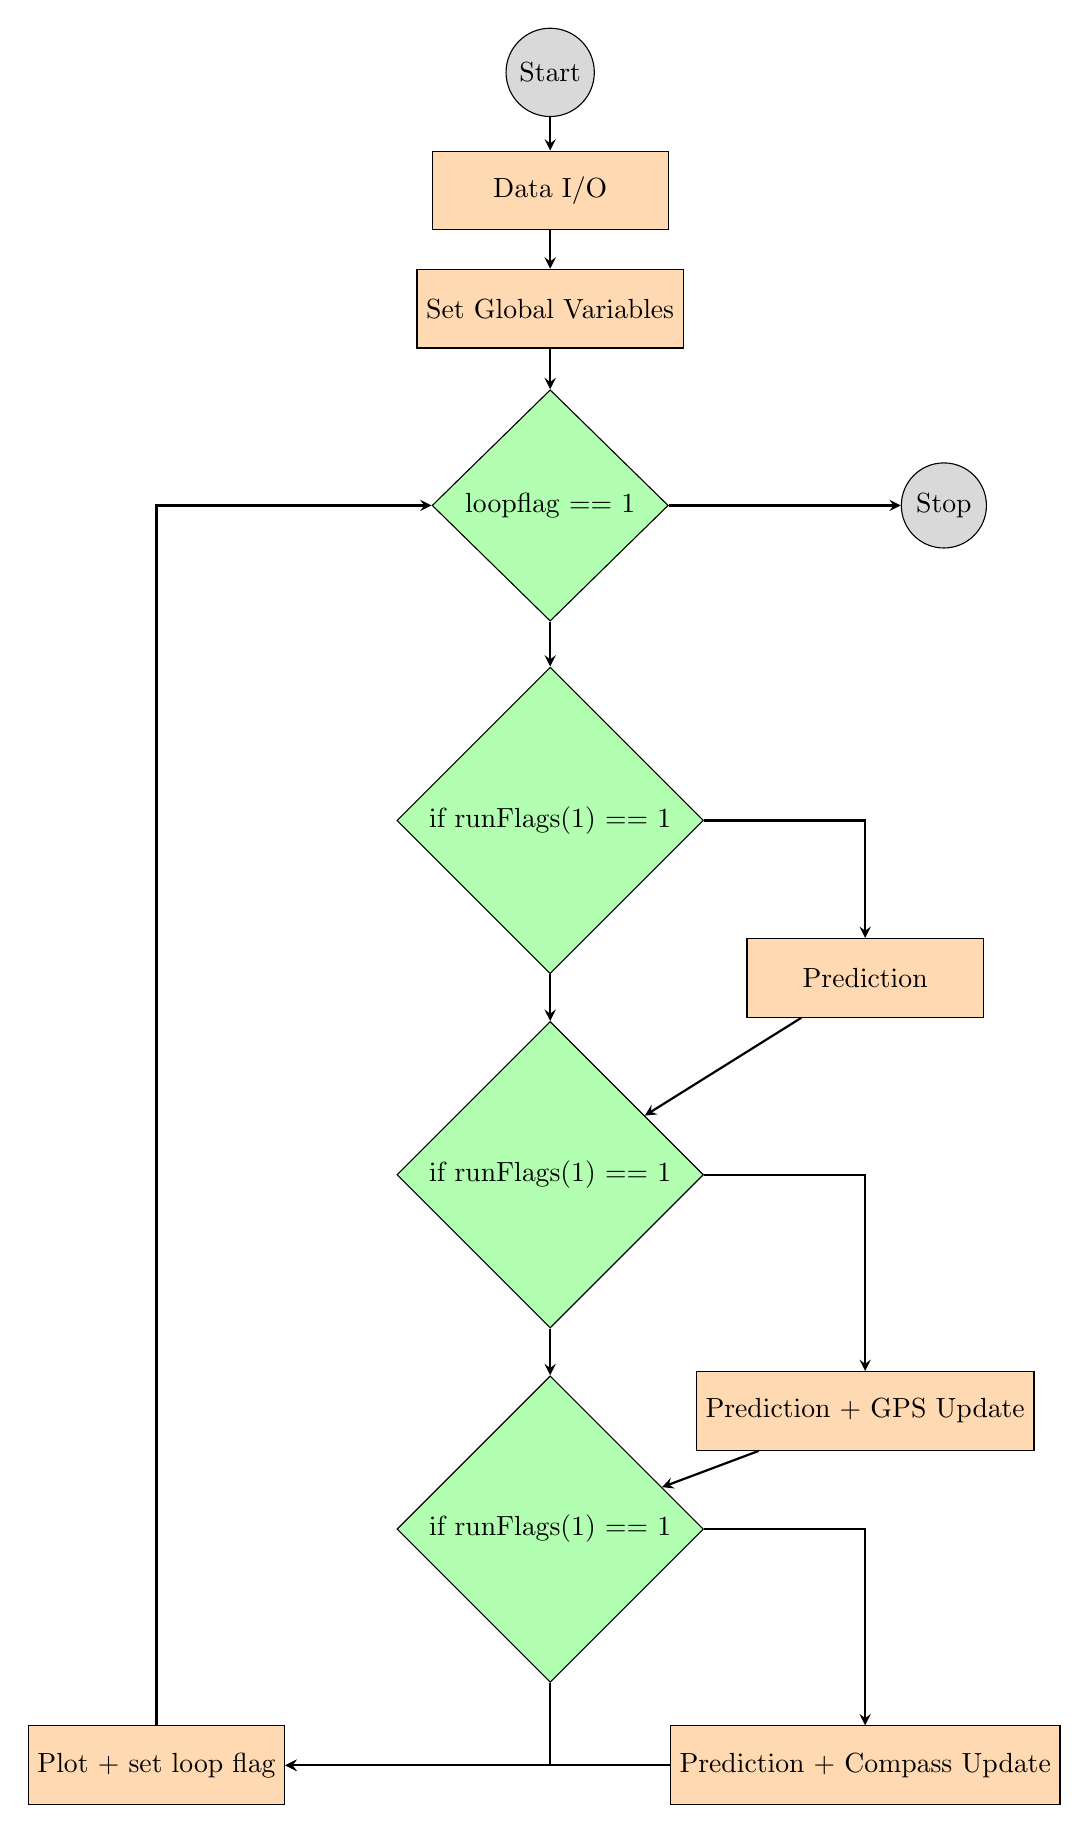
\begin{tikzpicture}[node distance = 1cm]
				%\node(label)[type]{name}
				\node(start)[startstop]{Start};
				\node(dataio)[process, below of = start, yshift = -0.5cm]{Data I/O};
				\node(globals)[process, below of = dataio, yshift = -0.5cm]{Set Global Variables};
				
				\node(while)[decision, below of = globals, yshift = -1.5cm]{loopflag == 1};
				
				\node(if1)[decision, below of = while, yshift = -3cm]{if runFlags(1) == 1};
				\node(do1)[process, right of = if1, xshift = 3cm, yshift = -2cm]{Prediction};
				
				\node(if2)[decision, below of = if1, yshift = -3.5cm]{if runFlags(1) == 1};
				\node(do2)[process, below of = if2, xshift = 4cm, yshift = -2cm]{Prediction + GPS Update};
				
				\node(if3)[decision, below of = if2, yshift = -3.5cm]{if runFlags(1) == 1};
				\node(do3)[process, below of = if3, xshift = 4cm, yshift = -2cm]{Prediction + Compass Update};
				
				\node(plot)[process, left of = do3, xshift = -8cm]{Plot + set loop flag};
				
				\node(stop)[startstop, right of = while, xshift = 4cm]{Stop};
				
				%arrows
					\draw [arrow] (start) -- (dataio);
					\draw [arrow] (dataio) -- (globals);
					\draw [arrow] (globals) -- (while);
					\draw [arrow] (while) -- (if1);
					\draw [arrow] (if1) -| (do1);
					\draw [arrow] (if1) -- (if2);
					\draw [arrow] (do1) -- (if2);
					\draw [arrow] (if2) -| (do2);
					\draw [arrow] (if2) -- (if3);
					\draw [arrow] (do2) -- (if3);
					\draw [arrow] (if3) -| (do3);
					\draw [arrow] (if3) |- (plot);
					\draw [arrow] (do3) -- (plot);
					\draw [arrow] (plot) |- (while);
					\draw [arrow] (while) -- (stop);
										

			%	\node(stop)[startstop, below of = obsDataStruct, yshift = -1cm, xshift = -5cm]{Stop};
				\end{tikzpicture}
				\caption[\textit{A3}]{Overall Program Flow\label{DIOP}}
			\end{centering}
		\end{figure}
		
		
		
		
		\pagebreak
		\subsubsection{Data I/O}
			Having to store each set of data separately while still having easily accessible data (for ease of writing the code and minimization of code runtime) we needed to filter the data into a series of structural arrays with the following template:
			$$Observation Data Structure =
			\begin{bmatrix}
			timestampVel (s) & timestampGPS & timestampComp & timestamp... & measurement n\\
			\end{bmatrix}
			$$
			Process Descriptions:
			\newcounter{listcounter}
			\begin{list}{\arabic{listcounter})~}{\usecounter{listcounter}}
				\item Parse Input: Takes in the columns of data with space delimiting input saving the first column to "Seconds", second column to "Microseconds", and each subsequent observation column into a Measurements vector. In Figure~\ref{DIOP} we see the structural flow for an 2-parameter data set such as Velocity Observations where Velocity would be Measurements 1 and Turn Rate would be Measurements 2.
				\item Merge Time Stamps: An implementation of the following equation: $ts1+ts2^{10-6} - First Time Stamp$\\
				This effectively "zeroes" the events so that the very first event occurs at $t = 0$		
			\end{list}
			
			\begin{figure}[position = here]
				\begin{centering}
					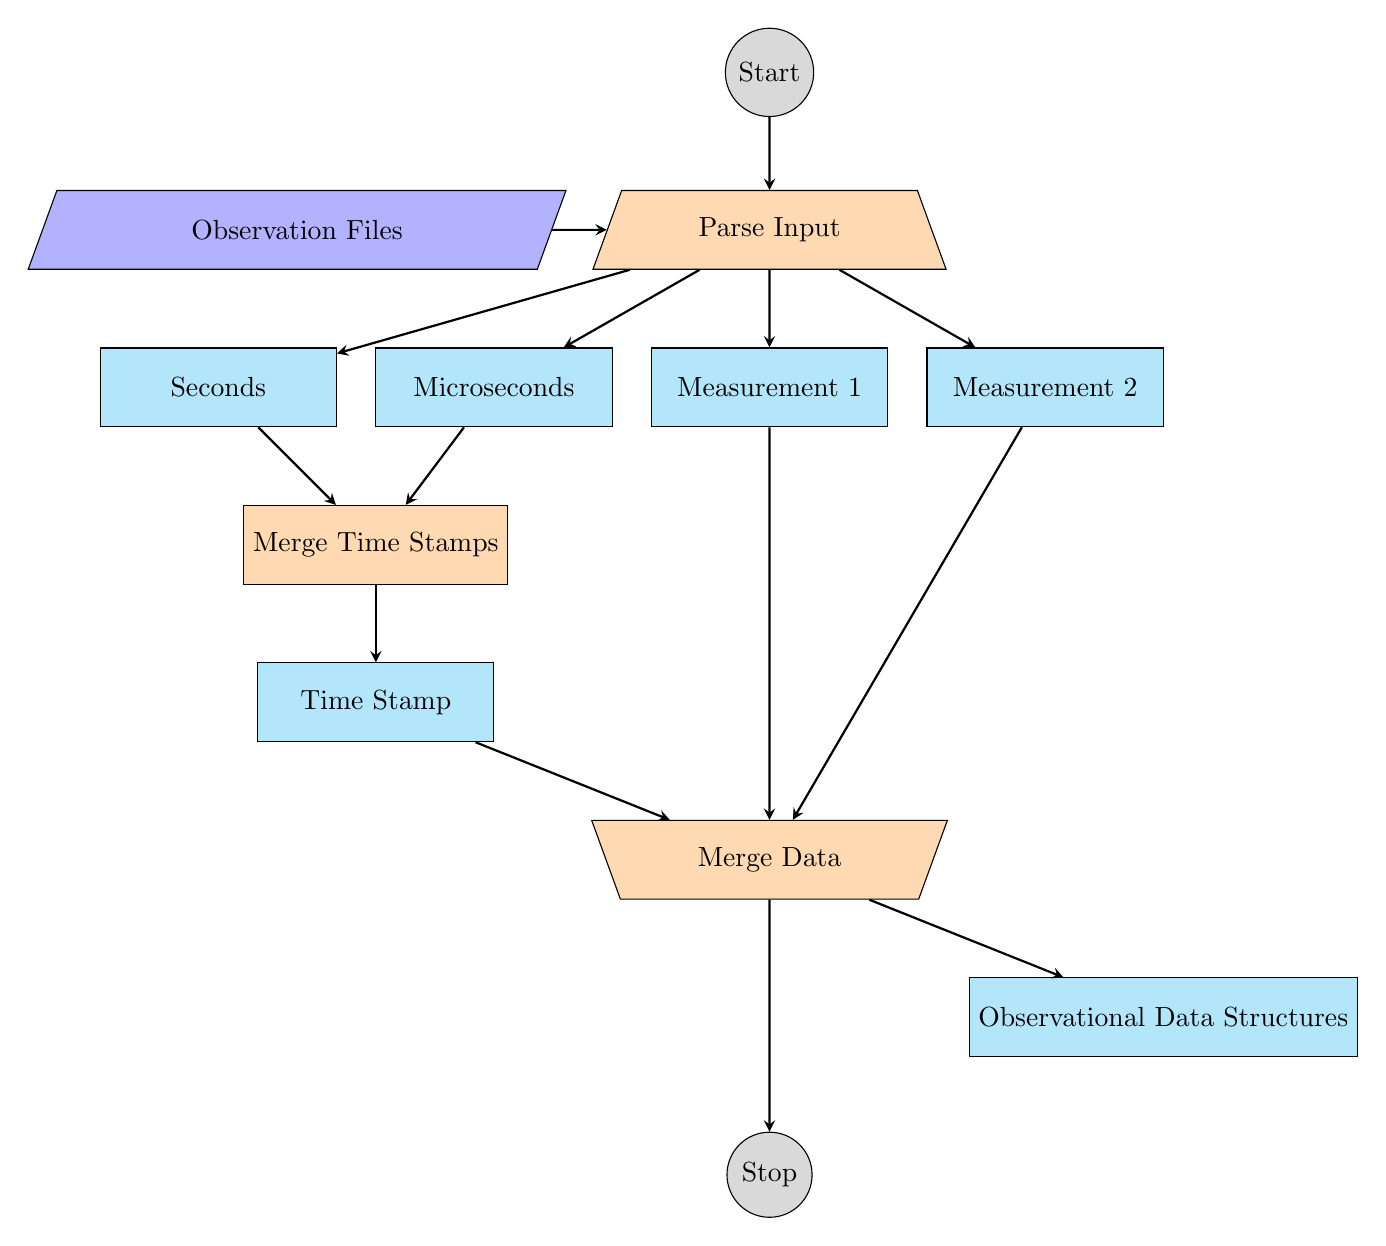
\begin{tikzpicture}[node distance = 1cm]
					%\node(label)[type]{name}
					\node(start)[startstop]{Start};
					\node(inParse1)[filtersplit, below of = start, yshift = -1cm]{Parse Input};
					\node(obsFile)[io, left of = inParse1, xshift = -5cm]{Observation Files};
					\node(values1)[datastruct, below of = inParse1, yshift = -1cm]{Measurement 1};
					\node(values2)[datastruct, right of = values1, xshift = 2.5cm]{Measurement 2};
					\node(ts2)[datastruct, left of = values1, xshift = -2.5cm]{Microseconds};
					\node(ts1)[datastruct, left of = ts2, xshift = -2.5cm]{Seconds};
					\node(mergets)[process, below of = ts2, yshift = -1cm, xshift = -1.5cm]{Merge Time Stamps};
					\node(timestamp)[datastruct, below of = mergets, yshift = -1cm]{Time Stamp};
					\node(mergedata)[filter, below of = timestamp, yshift = -1cm, xshift = 5cm]{Merge Data};
					\node(obsDataStruct)[datastruct,below of = mergedata, yshift = -1cm, xshift = 5cm]{Observational Data Structures};
					\node(stop)[startstop, below of = obsDataStruct, yshift = -1cm, xshift = -5cm]{Stop};
					
					\draw [arrow] (start) -- (inParse1);
					\draw [arrow] (obsFile) -- (inParse1);
					\draw [arrow] (inParse1) -- (ts1);
					\draw [arrow] (inParse1) -- (ts2);
					\draw [arrow] (inParse1) -- (values1);
					\draw [arrow] (inParse1) -- (values2);
					\draw [arrow] (ts1) -- (mergets);
					\draw [arrow] (ts2) -- (mergets);
					\draw [arrow] (mergets) -- (timestamp);
					\draw [arrow] (timestamp) -- (mergedata);
					\draw [arrow] (values1) -- (mergedata);
					\draw [arrow] (values2) -- (mergedata);
					\draw [arrow] (mergedata) -- (obsDataStruct);
					\draw [arrow] (mergedata) -- (stop);
					\end{tikzpicture}
				\caption[\textit{A3}]{Data I/O Process\label{DIOP}}
				\end{centering}
			\end{figure}
		
	\subsection{Prediction Stage Implementation}

		\pagebreak
	\subsection{Observation Stage Implementation}

		\pagebreak
	\subsection{Update Stage Implementation}



		\pagebreak
	\subsection{Code Listing}
		\subsubsection{Demonstration Code}
			\lstinputlisting{./code/dataFusionV3.m}
			\pagebreak
		\subsubsection{Development Code}
			This code listing includes a partially complete implementation of fusing the data from the Laser Range Finder detection of retro reflective beacons.
			\lstinputlisting{./code/dataFusion_v4.m}
			\pagebreak
	\section{Question 2}
	


	
	\subsection{Validity Check}
		\subsubsection{$R_{1}$}
	
			
		\pagebreak
		\subsubsection{$R_{2}$}
			
		\subsubsection{$R_{3}$}
		
		\subsubsection{$R_{4}$}
			
						
	\newpage
	\subsection{Roll/Pitch/Yaw Angles}

	\subsection{Angle Estimation}
	
	\subsection*{Code Listing}
	See Appendix A [9.2]
	\newpage
\section{Question 3}
\lstinputlisting{./MATLABFiles/q2.m}
	\pagebreak
	\subsection*{DH Notation}
	\noindent
		\begin{table}[position = here]
		\begin{centering}
		\begin{tabular}{||l|l|l|l|l||}
			\hline \rule[-2ex]{0pt}{5.5ex} \color{red}\bf{i} & \color{red}\bf{$\theta$}		&	\color{red}\bf{d}	&	\color{red}\bf{r}	&	\color{red}\bf{$\alpha$}\\ 
			\hline \rule[-2ex]{0pt}{5.5ex} 1 & $\theta_{1}$	&	67	&	100	&	$\pi/2$	\\	
			\hline \rule[-2ex]{0pt}{5.5ex} 2 & $\theta_{2}$	&	0	&	250	&	0		\\
			\hline \rule[-2ex]{0pt}{5.5ex} 3 & $\theta_{2}$	&	0	&	0	&	$\pi/2$	\\
			\hline \rule[-2ex]{0pt}{5.5ex} 4 & $\theta_{4}$	&	0	&	250	&	$-\pi/2$ \\
			\hline \rule[-2ex]{0pt}{5.5ex} 5 & $\theta_{5}$	&	0	&	0	&	$-\pi/2$	\\
			\hline \rule[-2ex]{0pt}{5.5ex} 6 & $\theta_{6}$	&	0	&	245	&	0		\\
			\hline 
		\end{tabular}\\\\
		\end{centering}
		\begin{flushleft}
		\caption [DHVariables] {D-H Variable Notation}\\\\
		\end{flushleft}}
		\end{table}
		
		
		\begin{figure}[position = here]
			\begin{centering}
				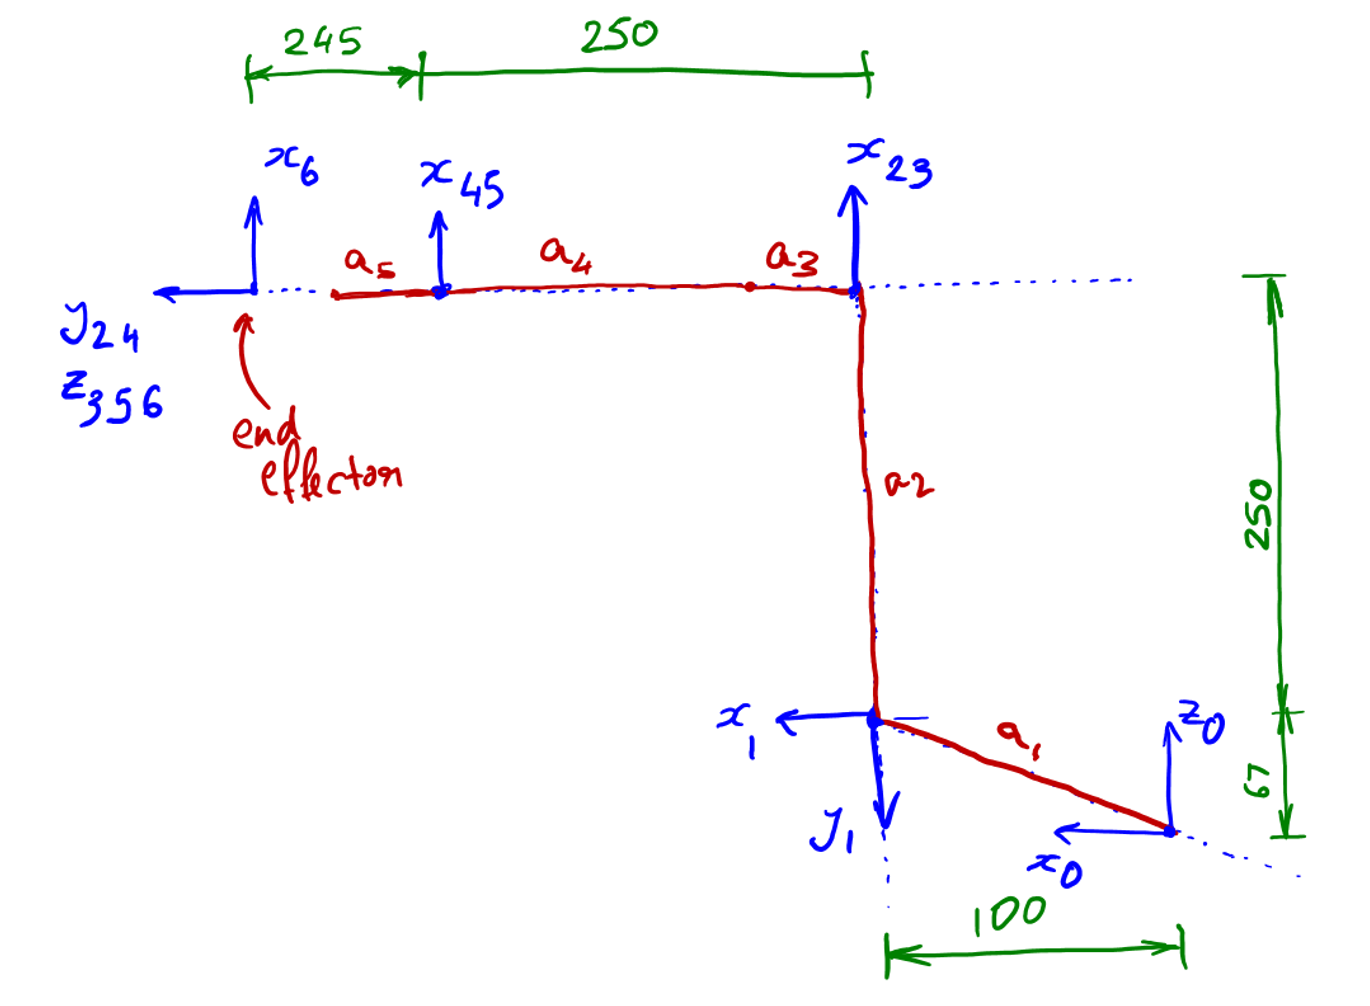
\includegraphics[scale=0.5]{q3}\\
				\caption [DHDrawing]{D-H Standard for Forward Kinematics Coordinate Systems}
			\end{centering}
		\end{figure}
		
	\pagebreak	
	\subsection*{Resulting Transformation Matrix}
	The resulting transformation matrix can be represented as:\\
		\begin{center}
			\bf{^{0}T_{6}} =
			\begin{pmatrix}
				n_{x} & s_{x} & a_{x} & p_{x}\\
				n_{y} & s_{y} & a_{y} & p_{y}\\
				n_{z} & s_{z} & a_{z} & p_{z}\\
				0	&	0	&	0	&	1
			\end{pmatrix}
			$ = {^{0}A_{1}}\mult{^{1}A_{2}}\mult{^{2}A_{3}}\mult{^{3}A_{4}}\mult{^{4}A_{5}}\mult{^{5}A_{6}}$
		\end{center}
		\vspace{5mm}
	\flushleft
\bf{n_{x}} =
$$
- \sin\theta_{6}\mult (\cos\theta_{4}\mult \sin\theta_{1} - \sin\theta_{4}\mult (\cos\theta_{1}\mult \sin\theta_{2}\mult \sin\theta_{3} - \cos\theta_{1}\mult \cos\theta_{2}\mult \cos\theta_{3}))-  \cos\theta_{6}\mult (\cos\theta_{5}\mult (\sin\theta_{1}\mult \sin\theta_{4} + \cos\theta_{4}\mult (\cos\theta_{1}\mult \sin\theta_{2}\mult \sin\theta_{3} - \cos\theta_{1}\mult \cos\theta_{2}\mult \cos\theta_{3})) + \sin\theta_{5}\mult (\cos\theta_{1}\mult \cos\theta_{2}\mult \sin\theta_{3} + \cos\theta_{1}\mult \cos\theta_{3}\mult \sin\theta_{2}))
$$\vspace{3mm}

\bf{s_{x}} = 
$$
\sin\theta_{6}\mult (\cos\theta_{5}\mult (\sin\theta_{1}\mult \sin\theta_{4} + \cos\theta_{4}\mult (\cos\theta_{1}\mult \sin\theta_{2}\mult \sin\theta_{3} - \cos\theta_{1}\mult \cos\theta_{2}\mult \cos\theta_{3})) + \sin\theta_{5}\mult (\cos\theta_{1}\mult \cos\theta_{2}\mult \sin\theta_{3} + \cos\theta_{1}\mult \cos\theta_{3}\mult \sin\theta_{2})) - \cos\theta_{6}\mult (\cos\theta_{4}\mult \sin\theta_{1} - \sin\theta_{4}\mult (\cos\theta_{1}\mult \sin\theta_{2}\mult \sin\theta_{3} - \cos\theta_{1}\mult \cos\theta_{2}\mult \cos\theta_{3}))
$$\vspace{3mm}


\bf{a_{x}} =
$$
\sin\theta_{5}\mult (\sin\theta_{1}\mult \sin\theta_{4} + \cos\theta_{4}\mult (\cos\theta_{1}\mult \sin\theta_{2}\mult \sin\theta_{3} - \cos\theta_{1}\mult \cos\theta_{2}\mult \cos\theta_{3})) - \cos\theta_{5}\mult (\cos\theta_{1}\mult \cos\theta_{2}\mult \sin\theta_{3} + \cos\theta_{1}\mult \cos\theta_{3}\mult \sin\theta_{2})
$$\vspace{3mm}

\bf{p_{x}} = 
$$
100\mult \cos\theta_{1} + 250\mult \cos\theta_{1}\mult \cos\theta_{2} - 250\mult \sin\theta_{1}\mult \sin\theta_{4} - 250\mult \sin\theta_{6}\mult (\cos\theta_{4}\mult \sin\theta_{1} - \sin\theta_{4}\mult (\cos\theta_{1}\mult \sin\theta_{2}\mult \sin\theta_{3} - \cos\theta_{1}\mult \cos\theta_{2}\mult \cos\theta_{3})) - 250\mult \cos\theta_{6}\mult (\cos\theta_{5}\mult (\sin\theta_{1}\mult \sin\theta_{4} + \cos\theta_{4}\mult (\cos\theta_{1}\mult \sin\theta_{2}\mult \sin\theta_{3} - \cos\theta_{1}\mult \cos\theta_{2}\mult \cos\theta_{3})) + \sin\theta_{5}\mult (\cos\theta_{1}\mult \cos\theta_{2}\mult \sin\theta_{3} + \cos\theta_{1}\mult \cos\theta_{3}\mult \sin\theta_{2})) - 250\mult \cos\theta_{4}\mult (\cos\theta_{1}\mult \sin\theta_{2}\mult \sin\theta_{3} - \cos\theta_{1}\mult \cos\theta_{2}\mult \cos\theta_{3})
$$\vspace{3mm}

\bf{n_{y}} =
$$
\sin\theta_{6}\mult (\cos\theta_{1}\mult \cos\theta_{4} + \sin\theta_{4}\mult (\sin\theta_{1}\mult \sin\theta_{2}\mult \sin\theta_{3} - \cos\theta_{2}\mult \cos\theta_{3}\mult \sin\theta_{1})) + \cos\theta_{6}\mult (\cos\theta_{5}\mult (\cos\theta_{1}\mult \sin\theta_{4} - \cos\theta_{4}\mult (\sin\theta_{1}\mult \sin\theta_{2}\mult \sin\theta_{3} - \cos\theta_{2}\mult \cos\theta_{3}\mult \sin\theta_{1})) - \sin\theta_{5}\mult (\cos\theta_{2}\mult \sin\theta_{1}\mult \sin\theta_{3} + \cos\theta_{3}\mult \sin\theta_{1}\mult \sin\theta_{2}))
$$\vspace{3mm}



\bf{s_{y}} =
$$
\cos\theta_{6}\mult (\cos\theta_{1}\mult \cos\theta_{4} + \sin\theta_{4}\mult (\sin\theta_{1}\mult \sin\theta_{2}\mult \sin\theta_{3} - \cos\theta_{2}\mult \cos\theta_{3}\mult \sin\theta_{1})) - \sin\theta_{6}\mult (\cos\theta_{5}\mult (\cos\theta_{1}\mult \sin\theta_{4} - \cos\theta_{4}\mult (\sin\theta_{1}\mult \sin\theta_{2}\mult \sin\theta_{3} - \cos\theta_{2}\mult \cos\theta_{3}\mult \sin\theta_{1})) - \sin\theta_{5}\mult (\cos\theta_{2}\mult \sin\theta_{1}\mult \sin\theta_{3} + \cos\theta_{3}\mult \sin\theta_{1}\mult \sin\theta_{2}))
$$\vspace{3mm}

\bf{a_{y}} = 
$$
- \sin\theta_{5}\mult (\cos\theta_{1}\mult \sin\theta_{4} - \cos\theta_{4}\mult (\sin\theta_{1}\mult \sin\theta_{2}\mult \sin\theta_{3} - \cos\theta_{2}\mult \cos\theta_{3}\mult \sin\theta_{1})) - \cos\theta_{5}\mult (\cos\theta_{2}\mult \sin\theta_{1}\mult \sin\theta_{3} + \cos\theta_{3}\mult \sin\theta_{1}\mult \sin\theta_{2})
$$\vspace{3mm}

\bf{p_{y}} =
$$
100\mult \sin\theta_{1} + 250\mult \cos\theta_{2}\mult \sin\theta_{1} + 250\mult \cos\theta_{1}\mult \sin\theta_{4} + 250\mult \sin\theta_{6}\mult (\cos\theta_{1}\mult \cos\theta_{4} + \sin\theta_{4}\mult (\sin\theta_{1}\mult \sin\theta_{2}\mult \sin\theta_{3} - \cos\theta_{2}\mult \cos\theta_{3}\mult \sin\theta_{1})) - 250\mult \cos\theta_{4}\mult (\sin\theta_{1}\mult \sin\theta_{2}\mult \sin\theta_{3} - \cos\theta_{2}\mult \cos\theta_{3}\mult \sin\theta_{1}) + 250\mult \cos\theta_{6}\mult (\cos\theta_{5}\mult (\cos\theta_{1}\mult \sin\theta_{4} - \cos\theta_{4}\mult (\sin\theta_{1}\mult \sin\theta_{2}\mult \sin\theta_{3} - \cos\theta_{2}\mult \cos\theta_{3}\mult \sin\theta_{1})) - \sin\theta_{5}\mult (\cos\theta_{2}\mult \sin\theta_{1}\mult \sin\theta_{3} + \cos\theta_{3}\mult \sin\theta_{1}\mult \sin\theta_{2}))
$$\vspace{3mm}

\bf{n_{z}} = 
$$
\cos\theta_{6}\mult (\sin\theta_{5}\mult (\cos\theta_{2}\mult \cos\theta_{3} - \sin\theta_{2}\mult \sin\theta_{3}) + \cos\theta_{4}\mult \cos\theta_{5}\mult (\cos\theta_{2}\mult \sin\theta_{3} + \cos\theta_{3}\mult \sin\theta_{2})) - \sin\theta_{4}\mult \sin\theta_{6}\mult (\cos\theta_{2}\mult \sin\theta_{3} + \cos\theta_{3}\mult \sin\theta_{2})
$$\vspace{3mm}

\bf{s_{z}} = 
$$
- \sin\theta_{6}\mult (\sin\theta_{5}\mult (\cos\theta_{2}\mult \cos\theta_{3} - \sin\theta_{2}\mult \sin\theta_{3}) + \cos\theta_{4}\mult \cos\theta_{5}\mult (\cos\theta_{2}\mult \sin\theta_{3} + \cos\theta_{3}\mult \sin\theta_{2})) - \cos\theta_{6}\mult \sin\theta_{4}\mult (\cos\theta_{2}\mult \sin\theta_{3} + \cos\theta_{3}\mult \sin\theta_{2})
$$\vspace{3mm}

\bf{a_{z}} = 
$$
\cos\theta_{5}\mult (\cos\theta_{2}\mult \cos\theta_{3} - \sin\theta_{2}\mult \sin\theta_{3}) - \cos\theta_{4}\mult \sin\theta_{5}\mult (\cos\theta_{2}\mult \sin\theta_{3} + \cos\theta_{3}\mult \sin\theta_{2})
$$\vspace{3mm}

\bf{p_{z}} = 
$$
250\mult \sin\theta_{2} + 250\mult \cos\theta_{6}\mult (\sin\theta_{5}\mult (\cos\theta_{2}\mult \cos\theta_{3} - \sin\theta_{2}\mult \sin\theta_{3}) + \cos\theta_{4}\mult \cos\theta_{5}\mult (\cos\theta_{2}\mult \sin\theta_{3} + \cos\theta_{3}\mult \sin\theta_{2})) + 250\mult \cos\theta_{4}\mult (\cos\theta_{2}\mult \sin\theta_{3} + \cos\theta_{3}\mult \sin\theta_{2}) - 250\mult \sin\theta_{4}\mult \sin\theta_{6}\mult (\cos\theta_{2}\mult \sin\theta_{3} + \cos\theta_{3}\mult \sin\theta_{2}) + 67
$$\vspace{3mm}
		
	\newpage
\renewcommand{\thesubsection}{\thesection.\arabic{subsection}}
\section{Appendix A}
	\subsection{Question 1}
	\pagebreak
	
	\subsection{Question 2}
	
		\subsubsection{obtainObstacles}
		\lstinputlisting{./code/q2/q2_obtain_obstacles.m}
		\subsubsection{obtainObstacles_v2}
		\lstinputlisting{./code/q2/q2_obtain_obstacles_attempt2.m}
		\subsubsection{generateOccupancyGrid}
		\lstinputlisting{./code/q2/occupancy_grid.m}
		\pagebreak
	
	\subsection{Question 3}
		
		
	\subsection*{Code Listing}
	See Appendix A [9.1]
	\\
	
	\pagebreak
	
\end{document}